\section{Метод конечных разностей для расчета токоперенос через гетероструктуру}
Конечно-разностная схема уравнения Шредингера (\ref{eq:ShredM}) для ГС на рис.\ref{fig:RTHSModel} \cite{Moskaluk}:
\begin{equation}
	\psi_{i-1}\frac{m^{*}_{i+1}}{m^{*}_{i-1}} + \psi_{i}\bigg(  \frac{2\Delta^{2}m^{*}_{i+1}}{\hbar^{2}}(E-U_{i}) - \frac{m^{*}_{i+1}}{m^{*}_{i-1}} - 1 \bigg) + \psi_{i+1} = 0,
\end{equation}
\begin{conditions}
	$m^{*}_{i}$ & эффективная масса в точке $i$;\\
	$\psi_{i}$ & волновая функция в точке $i$;\\ 
	$E$ & энергия электрона;\\
	$U_{i}$ & потенциальная энергия в точке $i$;\\
	$\Delta$ & шаг сетки.
\end{conditions}

\begin{figure}
	\centering
	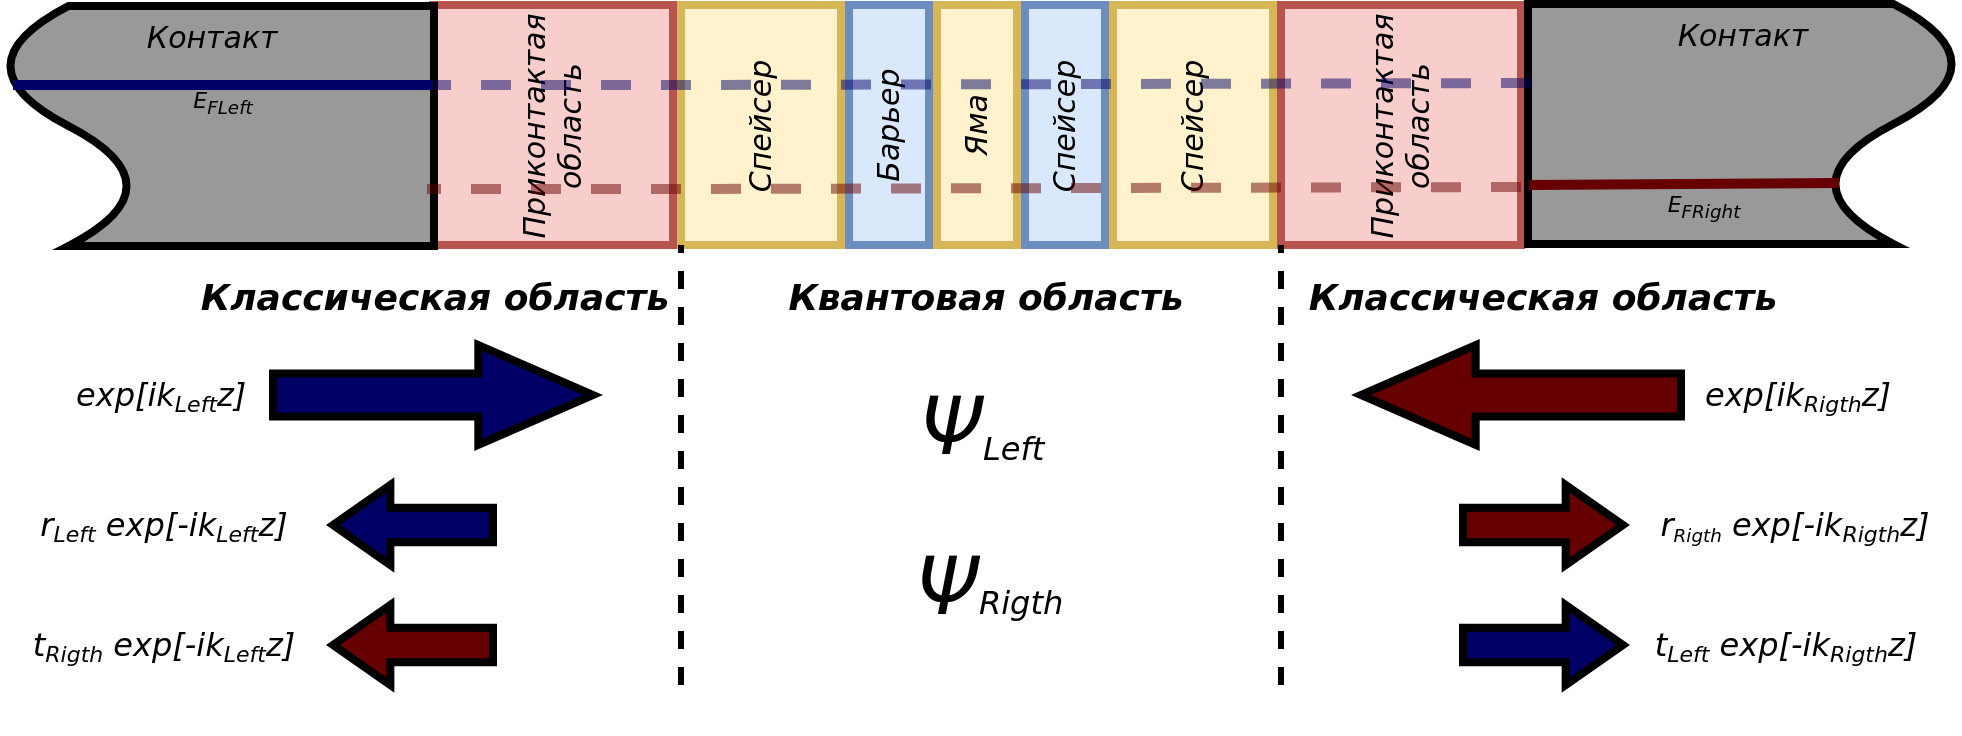
\includegraphics[width=1.08\linewidth]{RTHSModel}
	\caption{Схема модели РТГС}
	\label{fig:RTHSModel}
\end{figure}

Данное схема подходит для любой внутренней точки гетероструктуры, но не подходит для граничных точек. Граничные условия, для <<левых>> и <<правых>> электронов получаются из граничного условия Бастарда и вида волных функций в резервуарах:
\begin{gather}
	\begin{cases}
		(ik_{L}-1)\psi_{1} + \psi_{2} = 2ik_{L}\Delta;\\
		\psi_{N-1} + (ik_{R}\Delta - 1)\psi_{N} = 0;
	\end{cases}\\
	\begin{cases}
		(ik_{L}-1)\psi_{1} + \psi_{2} = 2ik_{L}\Delta;\\
		\psi_{N-1} + (ik_{R}\Delta - 1)\psi_{N} = 0;
	\end{cases}
\end{gather}
\begin{conditions}
	$k_{L(R)}$ & волновые функции в левом (правом) резервуаре.
\end{conditions}

\begin{lstlisting}[style=realcode,language=Matlab,caption={Алгоритм оценки дипломных работ}]
function [waveLeft, waveRigth] = getWaveFunction(delta, meff, U, Ez)
	hbar = 1.0551*1e-34;

	EzLen = length(Ez);
	ULen = length(U);

	waveLeft = zeros(EzLen, ULen);
	waveRigth = zeros(EzLen, ULen);

	for j = 1 : EzLen
		kLeft = sqrt( 2*meff(1)*(Ez(j) - U(1)) )/hbar;
		kRight = sqrt( 2*meff(end)*(Ez(j) - U(end)) )/hbar;

		d1 = ones(ULen-1, 1);
		d2 = 2*delta^2*meff(2:end-1).*( Ez(j)-U(2:end-1) )./hbar^2 - meff(2:end-1)./meff(3:end) - 1;
		d2 = [1i*kLeft*delta - 1, d2, 1i*kRight*delta - 1];
		d3 = [1, meff(2:end-1)./meff(3:end)];

		H = diag(d1, -1) + diag(d2) + diag(d3, +1);

		fLeft = [2*1i*kLeft*delta; zeros(ULen-1, 1)];
		fRight = [zeros(ULen-1, 1); 2*1i*kRight*delta];

		waveLeft(j, :) = (inv(H)*fLeft)';
		waveRigth(j, :) = (inv(H)*fRight)';
	end
	
end
\end{lstlisting}

\begin{lstlisting}[style=realcode,language=Matlab,caption={Алгоритм оценки дипломных работ}]
function val = TDEz(delta, meff, U, Ez, EFermi)
	hbar = 1.0551*1e-34;
	k_B = 1.38e-23;
	T = 300;
	kT = T*k_B;

	kLeft = abs( sqrt( 2*meff(1)*(Ez-U(1)) )/hbar );
	kRight = abs( sqrt( 2*meff(end)*(Ez-U(end)) )/hbar );

	[waveLeft, ~] = getWaveFunction(delta, meff, U, Ez);

	T = (kRight./kLeft).*(meff(1)/meff(end)).*(abs(waveLeft(:, end)).^2)';
	D = log( ( 1 + exp( (EFermi + U(1) - Ez)/kT ) ) ./ ( 1 + exp( (EFermi + U(end) - Ez)/kT ) ) );

	val = T.*D;
end
\end{lstlisting}

\begin{lstlisting}[style=realcode,language=Matlab,caption={Алгоритм оценки дипломных работ}]
function J = getJ(dx, meff, Ec, dU, EFermi, r, a, b, c)
	e = 1.6e-19; eVtoJ = e; JtoEv = e^(-1); 
	hbar = 1.054*1e-34; k_B = 1.38e-23;
	T = 300;
	kT = T*k_B;

	k = ((2*meff(1)*e*kT)/(4*pi^2*hbar^3));
	J = k*ones(1, length(dU));

	for j = 1:length(dU)
		Uj = Ec - linspace( 0, dU(j), length(Ec) );
		dTDEz = @(Ez) TDEz(dx, meff, Uj, Ez, EFermi);
		J(j) = J(j)*integral(dTDEz, 0, max(Uj), 'AbsTol', 1e-35);
	end
end
\end{lstlisting}